%!TeX root = SAS2017_18_senacheribbe.tex


\graphicspath{{graphics/task3/}}
\chapter{Task 3: filtering white Gaussian noise with discrete-time LTI filter}
\section{Description of the task}
The scope of this task is to generate a white Gaussian noise signal with $G_x=\frac{N_0}{2}$ and use it as input for the low-pass Butterworth filter of Task 2.\\
The variance of the output signal has to be measured for 5 different realizations of the input signal (10000 samples each), using the values for $N_0=[1, 10^{-5}, 10^{-10}, 10^{-15}, 10^{-20}]$. In the same plot, the measured variances should be compared with the theoretical variances of the response to an ideal WGN.\\
The histogram of the distribution for the values of one output with $N_0=1$ has to be presented. \\
Finally two realizations of the input with $N_0=1$ and 1000 samples should be plotted with the corresponding outputs.
\section{MATLAB code}
\lstinputlisting[style= Matlab-editor,  basicstyle=\small]{../final_project_task3.m}

\pagebreak
\section{Results and comments}
\subsection{Generation of white noise}
To generate a WGN we use the MATLAB command \textit{randn()}, which outputs a vector of normally distributed samples with $\mu=0$ and $\sigma^2_x=1$.
To obtain the requirement of $G_x=\frac{N_0}{2}$ in the frequency range $[-\frac{1}{2 \dt} \frac{1}{2 \dt}]$ we recall that
\begin{equation*}
P_x=\int_{-\frac{1}{2 \dt}}^{\frac{1}{2 \dt}} G_x(f)df = R_x(\tau=0)=\sigma^2_x
\end{equation*}
and by solving the integral we get the desired value for $\sigma^2_x$
\begin{equation}\label{eq:t3_sigma_req}
\sigma^2_x=\frac{N_0}{2 \dt}
\end{equation}
We can obtain the required signal by multiplying the vector generated with \textit{randn()} by the standard deviation $\sigma_x$ found in \cref{eq:t3_sigma_req}.
\subsection{Evaluation of the output}
The output of the filter has been evaluated using the implementation of Task 2. Two realizations for the input with $N_0=1$ (1000 sample) and the corresponding outputs are plotted in \cref{fig:t3_io_1,fig:t3_io_2}. \\
It can be noticed that the input has higher standard deviation ($\sigma_x\approx 10$) than the output ($\sigma_x\approx 1.8$), as we will compute analytically after.\\
The distribution of the values of the output for a realization with $N_0=1$ and 10000 sample is presented in the histogram in \cref{fig:t3_histogram}. The samples are Gaussian distributed as we can expect by filtering a Gaussian input with a LTI system.
\begin{figure}[H]
	\centering
	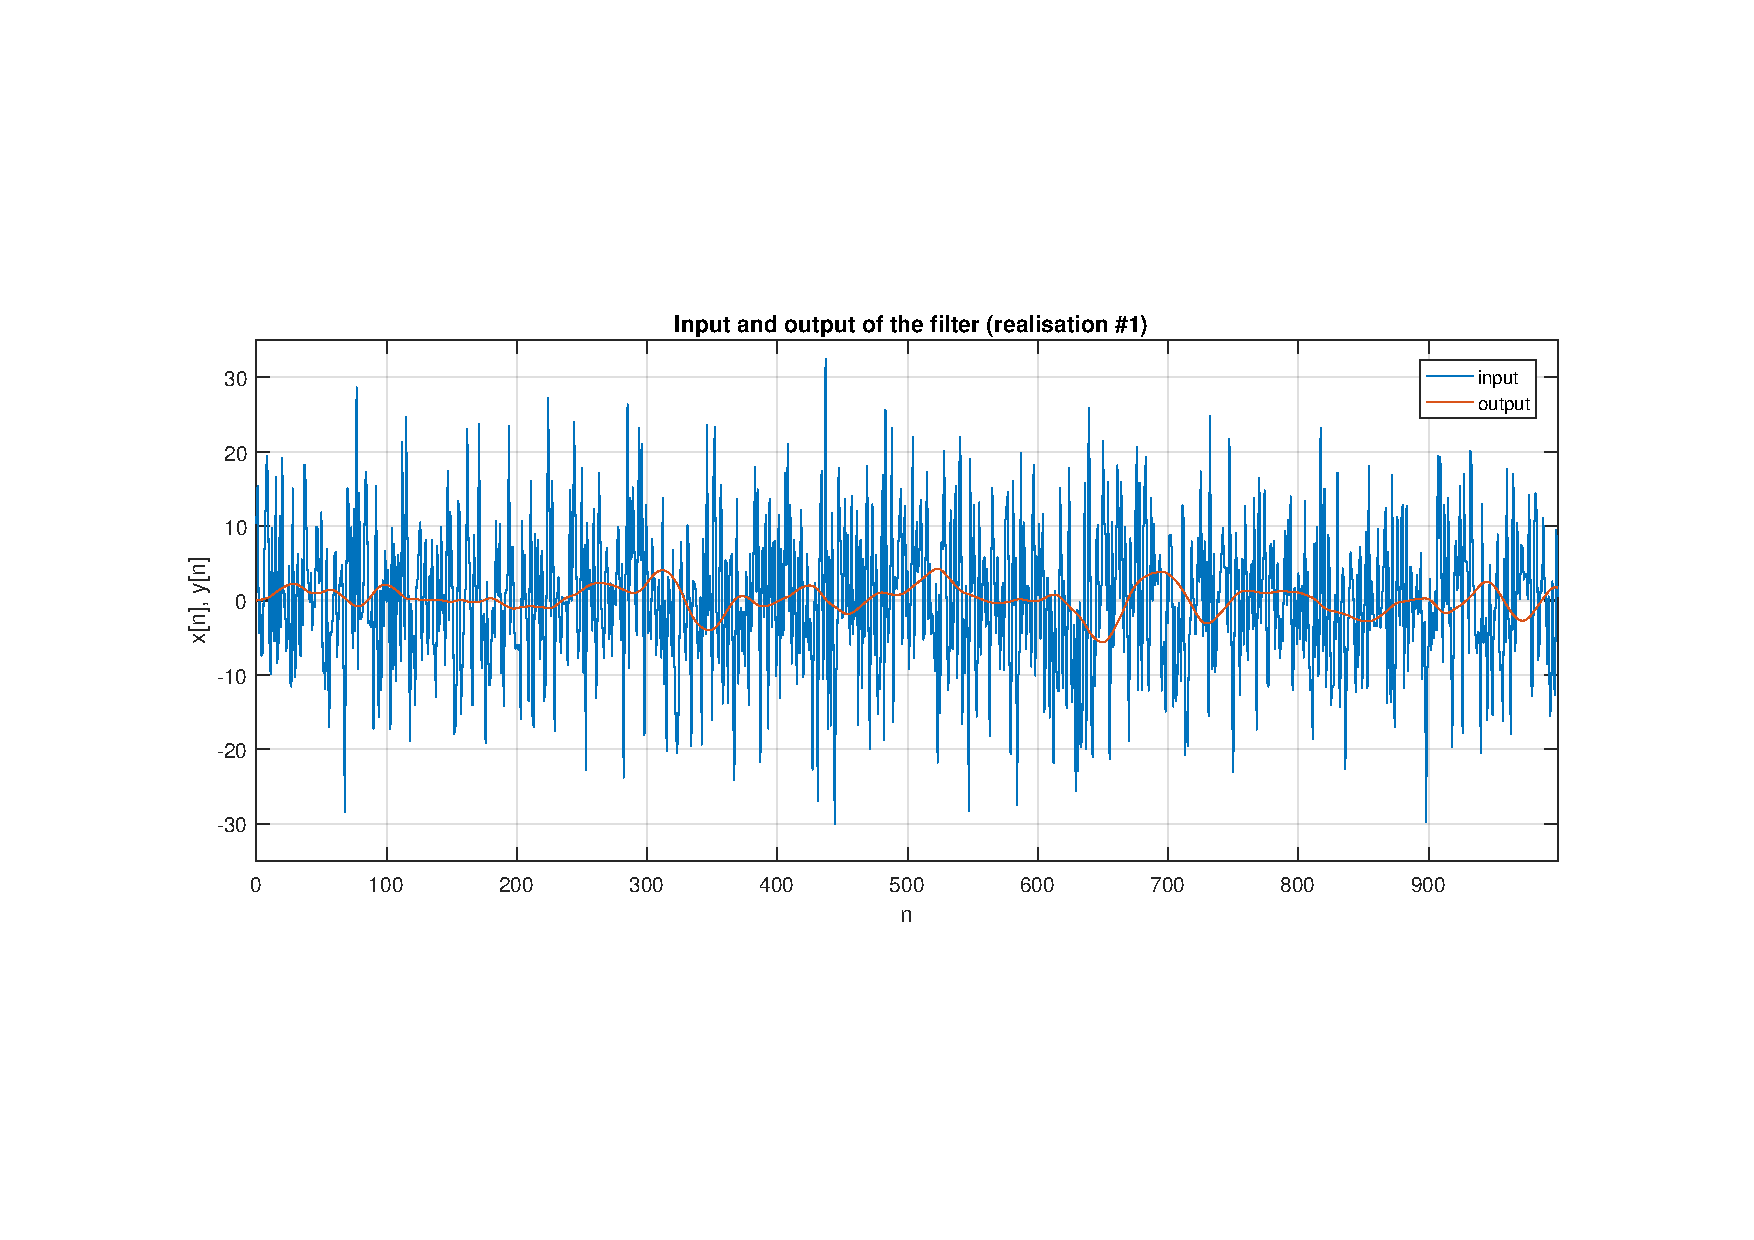
\includegraphics[trim={2.5cm 5cm 2.5cm 5cm}, clip, width=\linewidth]{io_1}
	\caption{Input and output of the filter (realization \#1)}
	\label{fig:t3_io_1}
\end{figure}

\begin{figure} [H]
	\centering
	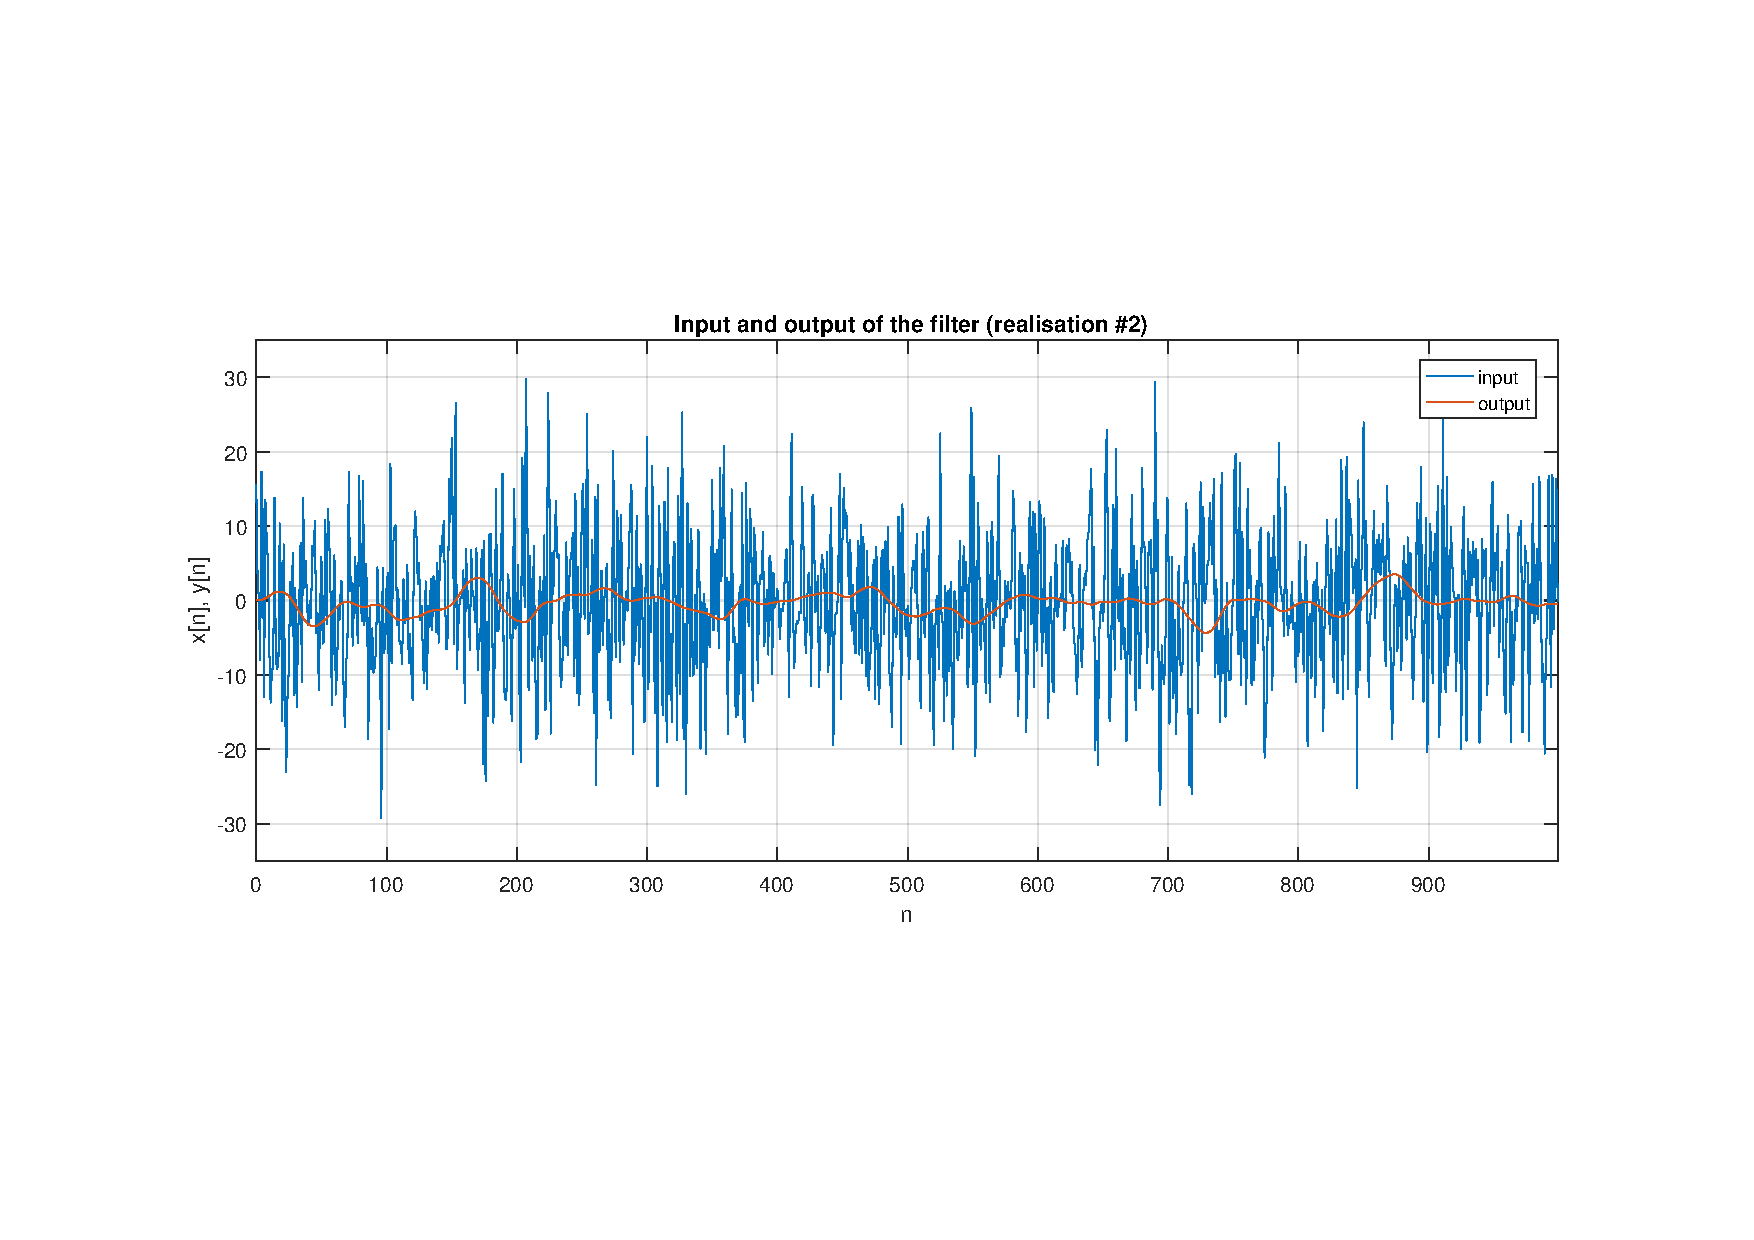
\includegraphics[trim={2.5cm 5cm 2.5cm 5cm}, clip, width=\linewidth]{io_2}
	\caption{Input and output of the filter (realization \#2)}
	\label{fig:t3_io_2}
\end{figure}
\begin{figure}[H]
	\centering
	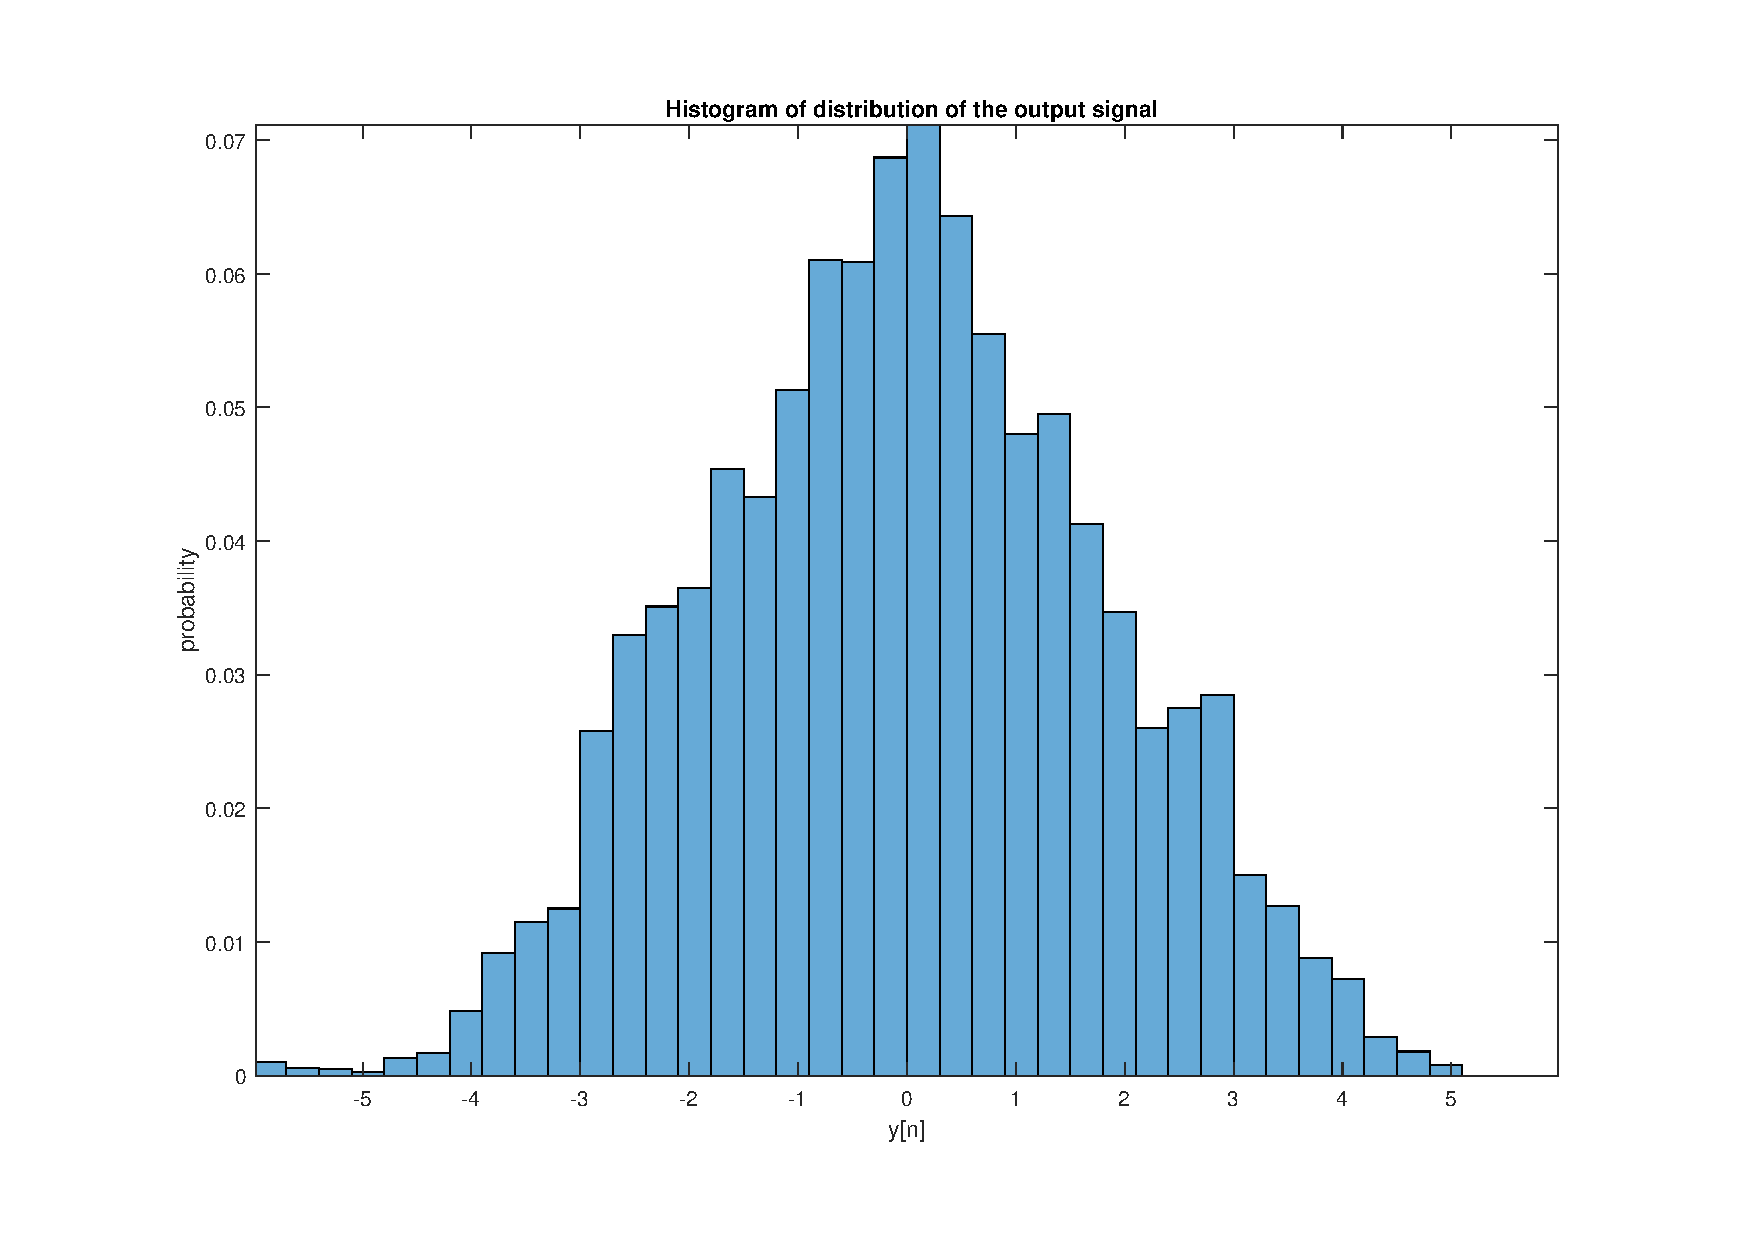
\includegraphics[trim={2.5cm 1.5cm 2.5cm 1.5cm}, clip, width=0.75\linewidth]{histogram}
	\caption{Histogram of distribution of the output signal  (10000 samples, $N_0=1$) - the output is Gaussian distributed with $\sigma\approx 1.8$}
	\label{fig:t3_histogram}
\end{figure}

\subsection{Variance of the output}
The mean value and the variance of the output of the filter can be derived analytically as
\begin{align}
\mu_y&=\cancelto{0}{\mu_x} \quad  H(0)=0\nn\\
\sigma^2_y&=E(Y^2(t))=\frac{N_0}{2} \mathcal{E} (h(t))=\frac{N_0}{2}\frac{20}{3}=N_0 \frac{10}{3} \label{eq:t3_theo_var}
\end{align}
In \cref{fig:t3_variances} the variances measured by evaluating the response of the filter (5 realizations for each value of $N_0$, 10000 samples each) are compared with the theoretical result in \cref{eq:t3_theo_var}. The result for $N_0=1$ is presented in detail in \cref{fig:t3_variances_zoom}. As we can see from both figures, the results are consistent with theory.
\begin{figure}[H]
	\centering
	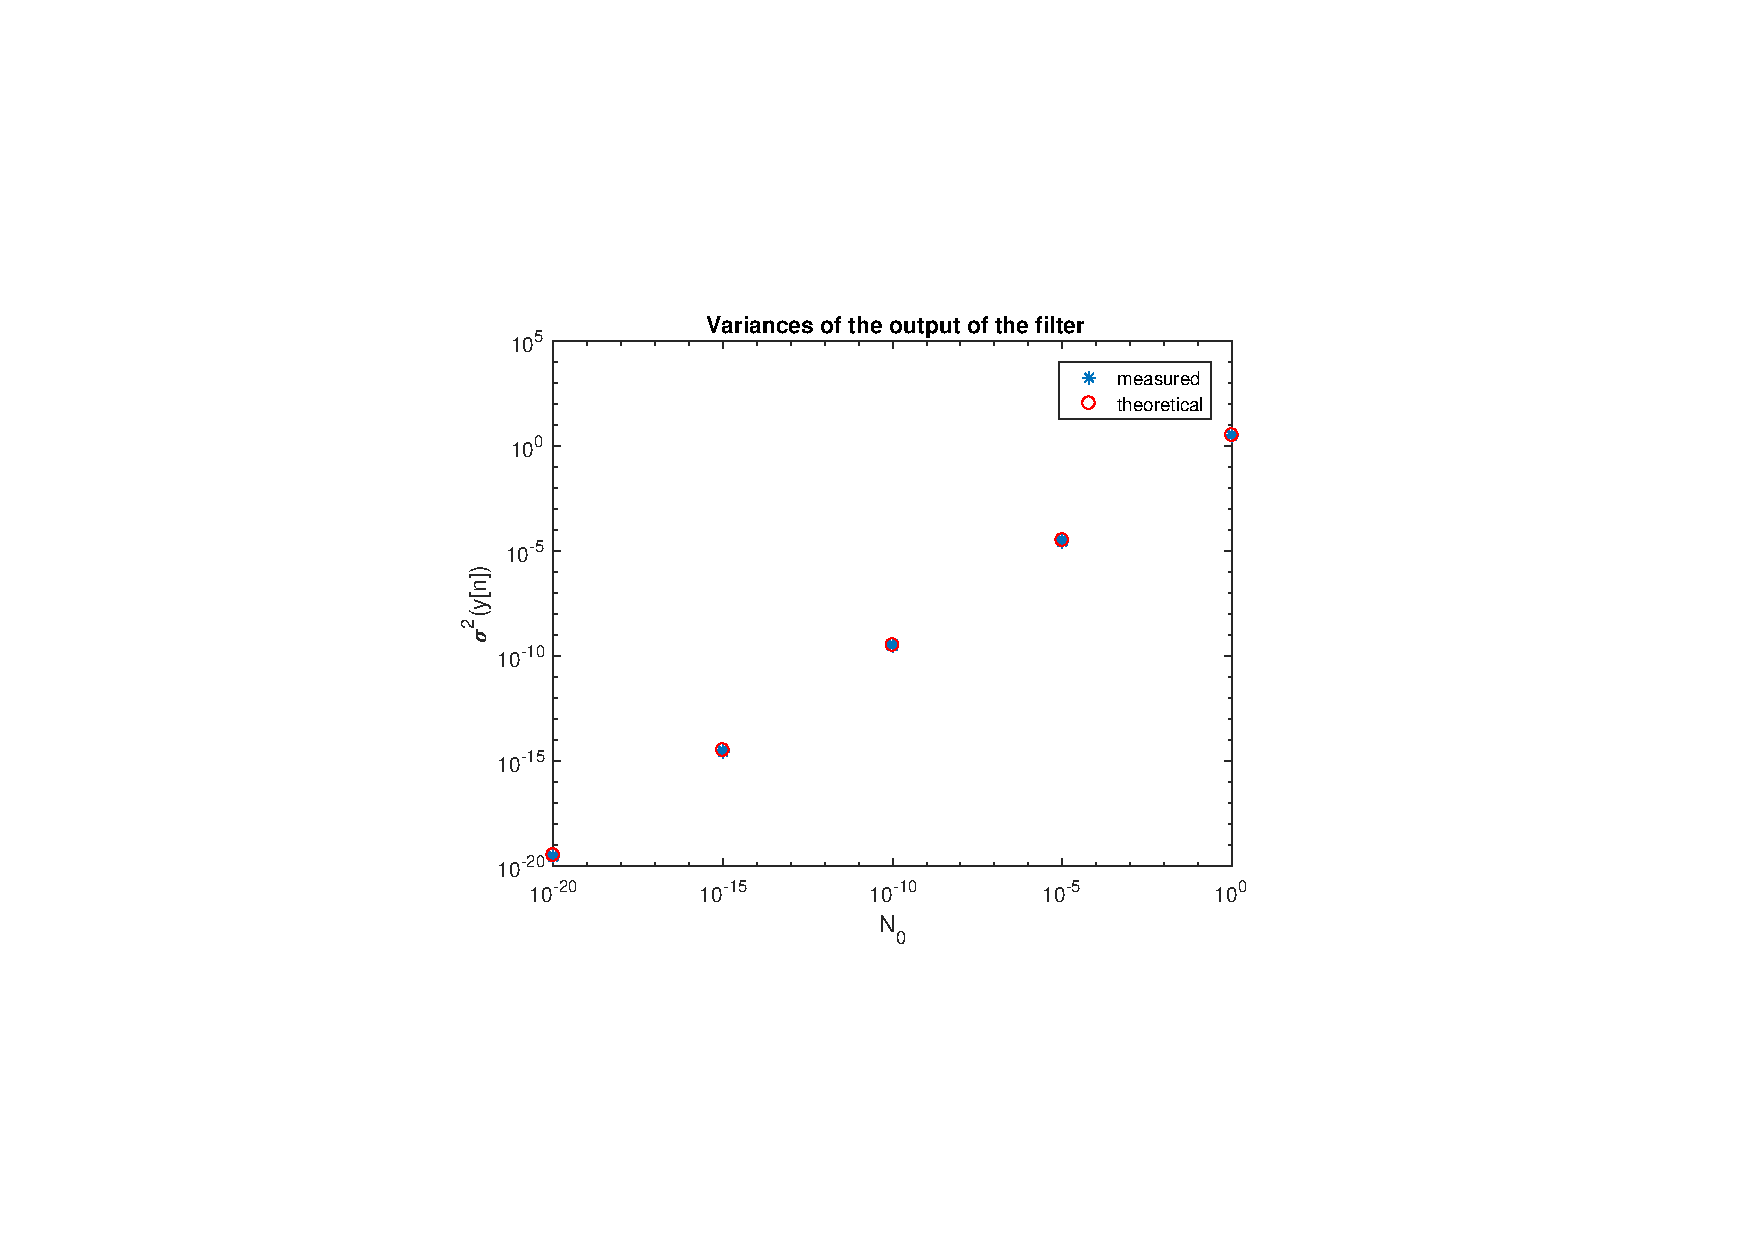
\includegraphics[trim={7.8cm 4.8cm 8cm 5cm}, clip, width=0.8\linewidth]{variances}
	\caption{Variances of the output of the filter - the results are consistent with theory}
	\label{fig:t3_variances}
\end{figure}
\begin{figure}[H]
\centering
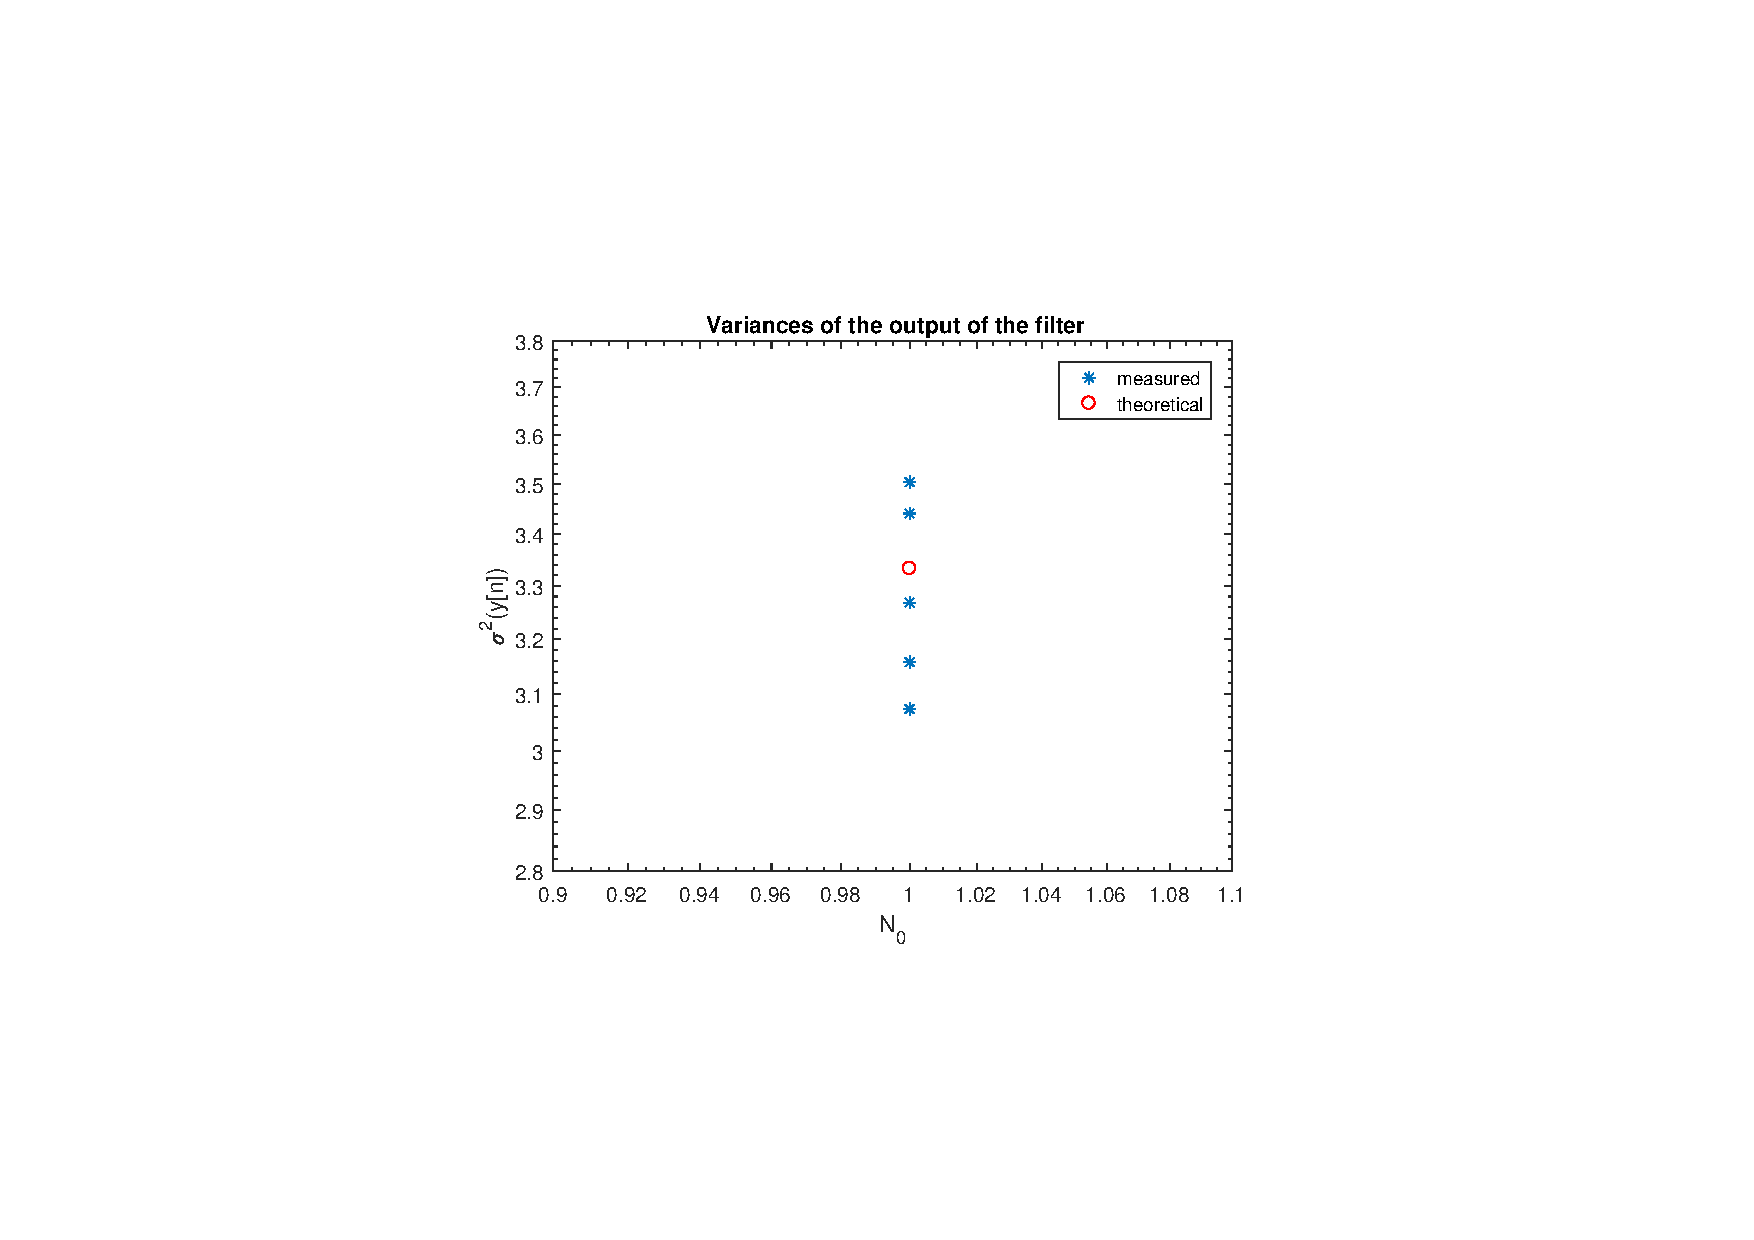
\includegraphics[trim={7.8cm 4.8cm 8cm 5cm}, clip, width=0.8\linewidth]{variances_zoom}
\caption{Variances of the output of the filter, zoom for $N_0=1$}
\label{fig:t3_variances_zoom}
\end{figure}
